% ------------------------------------------------------------------------------
% TYPO3 v9 LTS - What's New (German Version)
%
% @license	Creative Commons BY-NC-SA 3.0
% @link		https://typo3.org/help/documentation/whats-new/
% @language	German
% ------------------------------------------------------------------------------

\section{Backend User Interface}
\begin{frame}[fragile]
	\frametitle{Backend User Interface}

	\begin{center}\huge{\color{typo3darkgrey}\textbf{Backend User Interface}}\end{center}
	\begin{center}\large{\textit{The TYPO3 administration interface is now better than ever}}\end{center}

\end{frame}

% ------------------------------------------------------------------------------
% Page Tree

\begin{frame}[fragile]
	\frametitle{Backend User Interface}
	\framesubtitle{Seitenbaum}

	\begin{itemize}
		\item Der Seitenbaum basiert nun auf SVGs und bietet superschnelle Rendering-Zeiten
		\item Der gesamte ExtJS-Code wurde komplett aus dem TYPO3-Backend entfernt
		\item Seiten können ganz einfach gelöscht werden, indem sie nach rechts geschoben werden
	\end{itemize}

	\begin{figure}
		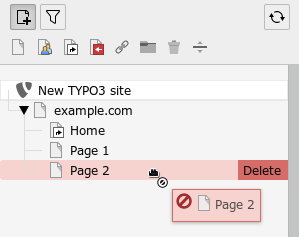
\includegraphics[width=0.3\linewidth]{BackendUserInterface/DeletePageInPageTree.png}
	\end{figure}

\end{frame}

% ------------------------------------------------------------------------------
% Page Tree

\begin{frame}[fragile]
	\frametitle{Backend User Interface}
	\framesubtitle{Modale Fenster}

	\begin{itemize}
		\item TYPO3 verwendet nun modale Fenster konsistent im Backend
		\item Dies gewährleistet eine reibungslose und unterbrechungsfreie Interaktion mit dem System
		\item So sieht das zum Beispiel beim Hinzufügen eines neuen Inhaltselements aus:
	\end{itemize}

	\begin{figure}
		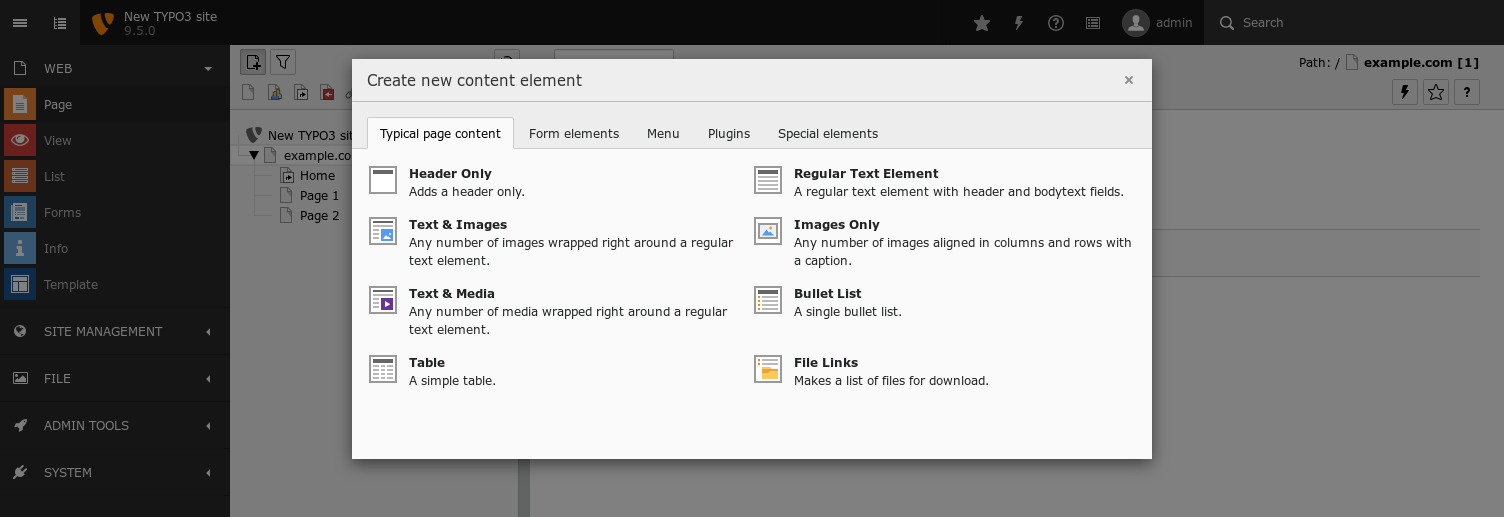
\includegraphics[width=0.85\linewidth]{BackendUserInterface/ModalWindowNewContentElement.png}
	\end{figure}

\end{frame}

% ------------------------------------------------------------------------------
% Duplicate Content Elements
% #84749 - Hide "duplicate" button by default

\begin{frame}[fragile]
	\frametitle{Backend User Interface}
	\framesubtitle{Duplizierte Inhaltselemente}

	% decrease font size for code listing
	\lstset{basicstyle=\smaller\ttfamily}

	\begin{itemize}
		\item Eine Schaltfläche zum Duplizieren eines Inhaltselements mit einem einzigen Mausklick wurde eingeführt
		\item Die Sichtbarkeit kann in userTSConfig konfiguriert werden ("1" = aktiviert):

\begin{lstlisting}
options.showDuplicate = 1
options.showDuplicate.[table] = 1
\end{lstlisting}

	\end{itemize}
	\vspace{-0.5cm}
	\begin{figure}
		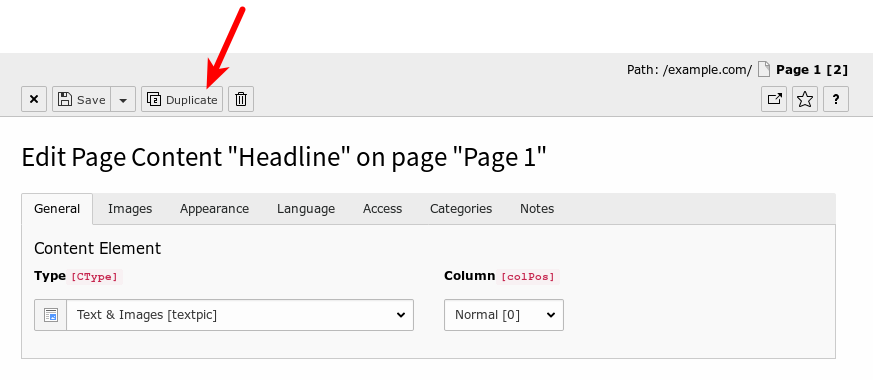
\includegraphics[width=0.8\linewidth]{BackendUserInterface/DuplicateButtonHiddenByDefault.png}
	\end{figure}

\end{frame}

% ------------------------------------------------------------------------------
% Further Improvements

\begin{frame}[fragile]
	\frametitle{Backend User Interface}
	\framesubtitle{Weitere Verbesserungen}

	\begin{itemize}
		\item TYPO3 berücksichtigt beim Bearbeiten des Bildes (z.B. Skalierung/Zuschneiden)
			die Bildausrichtung, die als EXIF-Angabe gespeichert ist
		\item Es wurden "Toggle-Schalter" eingeführt, die auch ein nützliches Werkzeug sind,
			um den einfachen Wechsel zwischen zwei Zuständen zu ermöglichen
		\item Vorschaubilder werden nun asynchron geladen\newline
			\small(zum Beispiel in der Dateiliste)\normalsize
		\item Im Debug-Modus wird den Admin-Benutzern der Name jedes FormEngine-Feldes im 
			Backend angezeigt\newline
			\small(siehe "Gründliche Änderungen" für ein Beispiel)\normalsize
		\item und viele andere Verbesserungen...
	\end{itemize}

\end{frame}

% ------------------------------------------------------------------------------
